\chapter{Diseño e Implementación}

	\section{Introducción}
	Debido a que se adoptó un modelo de desarrollo en espiral se plantearon una serie de prototipos que incluyen mayor funcionalidad en cada iteración
	del modelo. Inicialmente se planteó un prototipo básico para determinar factibilidad de puesta en funcionamiento de un SoC con microprocesador
	OpenRISC y el desarrollo de aplicaciones que se ejecuten en él. Debido a su funcionalidad reducida y menor consumo de recursos  para su síntesis se
	seleccionó el proyecto MinSoC para el desarrollo del primer prototipo con el cual se evaluaron y documentaron las capacidades del mismo, permitiendo
	valorar este proyecto para aplicaciones donde no se requieren grandes cantidades de memoria y juegan un papel primordial las entradas/salidas junto
	a la capacidad de procesamiento.  
		 
		\subsection{Entorno de ejecución}
		Actualmente OpenRISC es soportado por un conjunto de herramientas de desarrollo(toolchain) de 32 bits ofreciendo soporte para los lenguajes C y C++
		con librerías estáticas. El toolchain se encuentra disponible en dos formas: una para la ejecución de aplicaciones bajo el sistema operativo Linux y
		otra para la ejecución de aplicaciones standalone o bare metal que son aquellas que se ejecutan e interactúan directamente con el hardware sin la
		necesidad de un sistema operativo que proporcione soporte para la utilización de los periféricos.
		
			\subsubsection{Entorno de ejecución Standalone - Bare Metal}
	    	Para la ejecución de aplicaciones Bare Metal el toolchain se basa en la librería newlib que es una implementación estándar utilizada en
	    	sistemas embebidos. 
	    
			\subsubsection{Entorno de ejecución Linux}
			Por otro lado, para el uso de aplicaciones bajo el sistema operativo Linux el toolchain puede ser compilado en base a la librería uClibc que es la
			opción para sistemas embebidos de la librería glibc utilizada en los sistemas estándar.

		\subsection{Matriz de riesgo}
En cada prototipo se tienen en cuenta los posibles riesgos ya mencionadas y se amplían según la nueva visión del sistema.
		
		\subsection{Criterio para la realización de testing}%%corregir esto
		El testing desarrollado apunta a verificar el cumplimiento de los requerimientos individualmente e incrementalmente. Se pretende utilizar las
		aplicaciones de prueba provistas y desarrollar algunas que verfiquen los requerimientos de compilación, depuración y ejecución de aplicaciones para
		OpenRISC. 
		Los testing sirven para poder detectar la presencia de errores, pero aún si un testing no arroja resultados erróneos, esto no nos garantiza el
		correcto funcionamiento del sistema. El tipo de testing realizado es de verificación. La verificación es el proceso de evaluación de un sistema o
		componente para determinar si el producto cumple con lo que se ha diseñado, es decir, si cada fase de desarrollo dada cumple con los requisitos
		impuestos al inicio de dicha fase.

\chapter{Prototipo Uno : Implementación del SoC MinSoC en FPGA}

	\section{Introducción}
		
	En este primer prototipo se implementó el proyecto MinSoC en la placa de desarrollo S3ADSP1800A con el fin de verificar el funcionamiento del procesador y sus periféricos. Para lograr este objetivo se requiere de la instalación y puesta en funcionamiento de las herramientas de síntensis, place \& route(PAR) y programación de la FPGA Spartan 3A. 

	\section{Requerimientos del prototipo}
		\begin{table}[h]
		\centering
		\begin{tabular}{ p{2.5cm} p{8cm} p{3cm} }
		\hline 
		\rowcolor[gray]{0.8} N\textordmasculine Req & Descripción\\
		\hline 
		RQX-PA 1 & El prototipo debe implementar un SoC MinSoC en la placa desarrollo S3ADSP1800A\\ 
		\hline 
		RQX-PA 2 & El prototipo debe garantizar el correcto funcionamiento de todos los periféricos conectados al SoC mediante el bus Wishbone\\ 
		\hline 
		RQX-PA 3 & El prototipo debe interactuar correctamente con las interfaces hardware soportadas de la placa de desarrollo S3ADSP1800A\\ 
		\hline
		RQX-PA 4 & El prototipo debe ser capaz de ejecutar programas con capacidad de depuración generados mediante compilación
		cruzada en una arquitectura x86 y/o x86\_64 para la arquitectura OpenRISC\\
		\hline
		RQX-PA 5 & Se debe lograr depurar paso a paso y mediante break points las aplicaciones desarrolladas\\
		\hline		
		\end{tabular}
		\end{table}

\newpage
	
	\section{Matriz de Riesgo para el Prototipo Uno}

		\begin{table}[h!]
		\centering
		\begin{tabular}{ p{2.5cm} p{9cm} p{2cm} p{2cm} }
		\hline 
		\rowcolor[gray]{0.8} N\textordmasculine Req Asociados& Riegos Asociados & Severidad  & Ocurrencia \\
		\hline
		RQX-PA 1& EL código RTL disponible en la web tenga fallas reconocidas durante el proceso de síntesis & Crítica       & Probable \\
		\hline
				& Vencimiento de licencias de las herramientas privativas para el proceso de síntesis  & Menor  & Ocasional\\	 
		\hline
				& Falta de documentación de apoyo para la implentación
del Soc & Crítico & Ocasional\\	 
		\hline

		RQX-PA 2,RQX-PA 3 & Imposibilidad de acceso a alguno de los periféricos de la placa de desarrollo &  Catastrófico  & Probable\\
		\hline
		& Soporte de acceso a periféricos inexistente o con presencia
de bugs & Crítica  & Ocasional\\	 
		\hline
		RQX-PA 4& Compilación cruzada realizada con compiladores obsoletos & Severo  &  Ocasional\\ 
		\hline
		&Problemas en la compilación e instalación de las herramientas de desarrollo de software  & Severo  &  Ocasional\\ 
		\hline
		RQX-PA 5& Problemas con el driver provisto por el fabricante del  dispositivo programador JTAG -USB & Severo&  Ocasional\\
		\hline
		\end{tabular}
		\caption{Tabla de Riegos vs. Requerimientos}
		%\label{tab:riegos}
		\end{table}



		\begin{table}[h!]
		\centering
		\begin{tabular}{ p{4cm} p{4cm} p{4cm} p{3cm} }
		\hline 
		\rowcolor[gray]{0.8} Riesgo & Consecuencia & Estrategia preventiva & Estrategia de contingencia\\
		\hline
		EL código RTL disponible en la web tiene fallas reconocidas durante el proceso de síntesis.&Retraso en los tiempos de implementación.& Análisis previo de guías de resolución de problemas y preguntas frecuentes & Revisión de código y consulta a los desarrolladores \\
		\hline
		Vencimiento de licencias de las herramientas privativas para el proceso de síntesis & Imposibilidad de ejecución de las herramientas requeridas & Verificación previa de los vencimientos de las licencias & Renovación de licencia \\	 
		\hline
		Falta de documentación de apoyo para la implentación
del Soc& Perdida de tiempo en realizar la implementación
del SoC & Revisión previa de la documentación existente para la elección del
SoC & Dedicación de mayor tiempo para la implementación\\ 
		\hline
		 Imposibilidad de acceso a alguno de los periféricos de la placa de desarrollo & Imposibilitad de acceso a los periféricos del kit &Verificación previa de los recursos utilizados por el SoC a implementar & Depuración del codigo RTL del proyecto\\		
		\hline
		Problemas con el driver provisto por el fabricante del  dispositivo programador JTAG -USB  & Imposibilidad de configuración de la FPGA y depuración de aplicaciones &Análisis previo de los driver de los dispositivos a utilizar &  Utilización de dispositivos alternativos.\\		
		\hline
		\end{tabular}
		\caption{Planificación de riesgos}
		%\label{tab:planificación}
		\end{table}



		\newpage
		\section{Descripción de la Estructura del Prototipo Uno}
			

		La Figura ~\ref{fig:minsoc} muestra un diagrama de despliegue del prototipo planteado. Se utiliza un estación de trabajo corriendo las herramientas de compilación (GCC) y depuración (GDB) en sus versiones de compilación cruzada para arquitecturas destino OpenRISC. Se requiere de un
		servidor que proporcione un puerto para la depuración con GDB, acción realizada por la aplicación Advanced JTAG Bridge que provee la interfase de comunicación entre el TAP JTAG conectado al SoC a través el cable JTAG y la estación de trabajo.
		
		\begin{figure}[!h]
 		\begin{center}
  		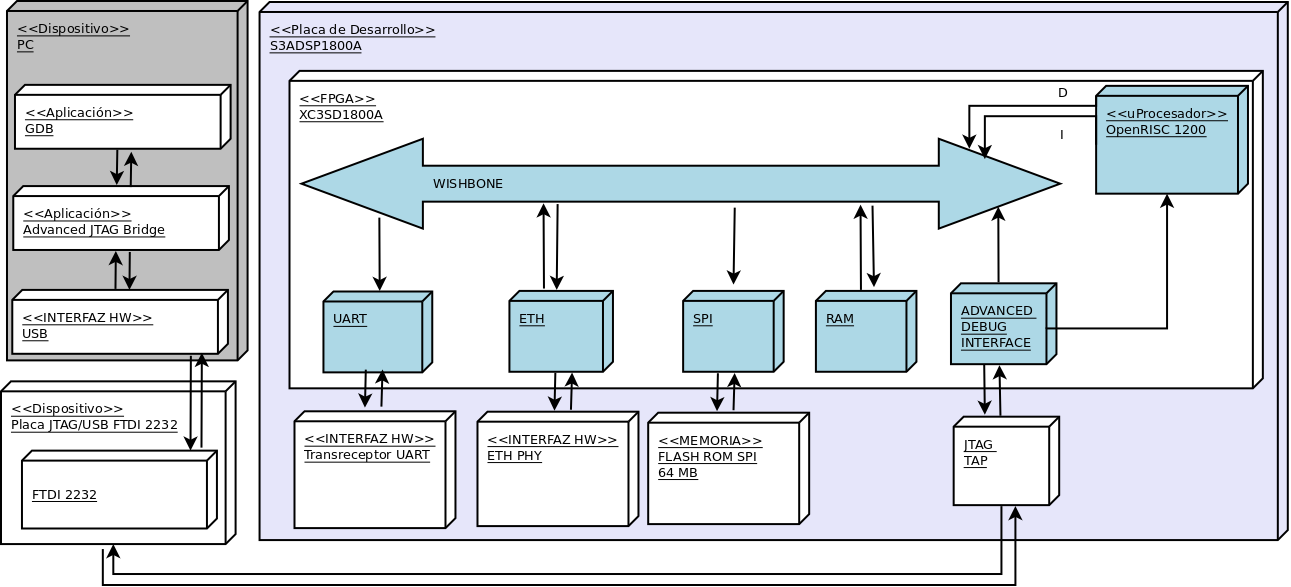
\includegraphics[width=1\textwidth,keepaspectratio=true]{./images/proto1}
  		\caption{Diagrama de despliegue Prototipo Uno}
  		\label{fig:minsoc}
 		\end{center}
		\end{figure}
		
		El módulo Advanced Debug Interface proporciona soporte para la depuración via JTAG, está conectado directamente al microprocesador y a su vez al bus
		general Wishbone donde se conectan el resto de los periféricos. Se conectan al sistema mediante el bus antes mencionado: un modulo	de RAM
		sintetizado, un módulo de arranque (startup), un módulo SPI que interactúa con la memoria flash on board de la placa S3ADSP1800A , un módulo UART y
		un módulo ETHERNET. El sistema inyecta un pequeño código de arranque directamente al bus de instrucciones al iniciar o luego de un reset. 

\newpage
			
		\section{Implementación}

La implementación se realiza normalmente en cinco pasos básicos: 
\begin {itemize}
\item Descarga del script de instalación.
\item Ejecución del script de instalación.
\item Configuración de la placa especifica para la síntesis.
\item Generación del flujo de bits.
\item Programación de la FPGA Spartan 3a.
 \end {itemize}
 Consulte la Guía de MinSoc en el Anexo 1 para la realización pasos a seguir en la implementación sobre la placa de desarrollo  S3ADSP1800A.
		
		%%%%%%%\subsection{Diagrama de Secuencia}
		%\subsection{Selección y Desarrollo de aplicaciones de prueba}
\newpage
		\section{Testing}

% Escribir sobre el testing del proto uno

\begin{table}[h!]
		\centering
		\begin{tabular}{ p{5cm} p{10cm}  }
		\hline 
	    \rowcolor[gray]{0.8}  Caso de Prueba&  Interactuar correctamente con las interfaz hardware UART\\
		\hline 
		Código de Requerimiento & RQX-PA 3\\ 
		\hline 
		Requerimiento  &  El prototipo debe interactuar correctamente con las interfaces hardware soportadas de la placa de desarrollo S3ADSP1800A\\ 
		\hline 
		Código de Testing & T001\\ 
		\hline
		Propósito & Comprobación del correcto funcionamiento de el componente UART \\
		\hline
		Realizado Por & Lovaisa Michelini, Valeria \\
		\hline	
		Entorno de Ejecución & Bare Metal \\
		\hline
		Precondiciones &  \begin {itemize}
							\item Instanciación en la FPGA del SoC.
							\item Ejecución de una terminal serie en la PC
							\item Comunicación establecida entre la placa de desarrollo y la PC
							\end {itemize}\\
		\hline
		Secuencia de Ejecución & Ejecutación de la aplicación de prueba uart.or32  \\
		\hline
		Postcondiciones & MinSoc corriendo sobre FPGA, lo que se manifiesta en la impresión de pantalla de la terminar remota en la PC\\
		\hline
 \multicolumn{2}{>{\columncolor[gray]{.8}}c}{Resultados}\\
		\hline
		Resultados Esperados & Poder observar por la terminal serial una cadena de string.\\
		\hline	
		Resultados Obtenidos & Al ejecutarse la aplicación de prueba del uart se pudo observar la cadena de string esperada "HELLO WORLD" \\
		\hline
		\end{tabular}
		\end{table}

\newpage
\begin{table}[h!]
		\centering
		\begin{tabular}{ p{5cm} p{10cm}  }
		\hline 
	\rowcolor[gray]{0.8}  Caso de Prueba&  Interactuar correctamente con las interfaces hardware de Ethernet\\
		\hline 
		Código de Requerimiento & RQX-PA 3\\ 
		\hline 
		Requerimiento  &  El prototipo debe Interactuar correctamente con las interfaces hardware soportadas de la placa de desarrollo S3ADSP1800A\\ 
		\hline 
		Código de Testing & T002\\ 
		\hline
		Propósito &  El envío de paquetes de Ethernet mediante broadcast desde el SoC  \\
		\hline
		Realizado Por & Gomez, Pablo \\
		\hline	
		Entorno de Ejecución & Bare Metal \\
		\hline
		Precondiciones & \begin {itemize}
							\item Instanciación en la FPGA del SoC.
							\item Ejecución de una terminal serie en la PC
							\item Ejecución de una aplicación snifer en la PC
							\item Comunicación establecida entre la placa de desarrollo y la PC
							\end {itemize} \\
		\hline
		Secuencia de Ejecución &  Ejecutación de la aplicación de prueba eth.or32\\
		\hline
		Postcondiciones &  MinSoc corriendo sobre FPGA, lo que se manifiesta en la impresión de pantalla de la terminar serie en la PC y en los paquetes captados por la aplicación wireshark \\
		\hline
 		\multicolumn{2}{>{\columncolor[gray]{.8}}c}{Resultados}\\
		\hline
		Resultados Esperados & Poder observar por la terminal serial una cadena de string indicando el inicio del envío de paquetes Ethernet y verificar la llegada de los mismos por medio de una aplicación sniffer \\
		\hline	
		Resultados Obtenidos & Al ejecutarse un programa de prueba pudo observarse la cadena de string "HELLO WORLD " y observar 0xFF02B4050 en los paquetes catados por la aplicación wireshark" \\
		\hline
		\end{tabular}
		\end{table}

%%%%%%%%%%%%%%%%%%%%%%%%%%%%%%%%%%%%%%%%%
\newpage
\begin{table}[h!]
		\centering
		\begin{tabular}{ p{5cm} p{10cm}  }
		\hline 
		\rowcolor[gray]{0.8}  Caso de Prueba& Ejecución de la aplicación multiplicadora de matrices binarias generadas mediante una Secuencia binaria pseudo aleatoria (PRBS) \\
		\hline 
		Código de Requerimiento & RQX-PA 4\\ 
		\hline 
		Requerimiento  &  El prototipo debe ser capaz de ejecutar programas con capacidad de depuración, generados mediante compilación cruzada en una arquitectura x86 y/o x86\_64 para arquitectura la OpenRISC\\ 
		\hline 
		Código de Testing & T003\\ 
		\hline
		Propósito &  Compilación y Ejecución de un  programa sencillo en c.Verificación de la capacidad de procesamiento del sistema mediante la realización de los productos con matrices cuadradas incrementando su tamaño iteración a iteración.  
\\
		\hline
		Realizado Por & Gomez, Pablo \\
		\hline	
		Entorno de Ejecución & Bare Metal \\
		\hline
		Precondiciones &\begin {itemize}
							\item Instanciación en la FPGA del SoC.
							\item Ejecución de una terminal serie en la PC
							\item Descarga e instalación del complicador cruzado 
							\item Comunicación establecida entre la placa de desarrollo y la PC
							\end {itemize}
 \\
		\hline
		Secuencia de Ejecución & Ejecución de la aplicación multiplicadora de matrices mult mat.or32 \\
		\hline
		Postcondiciones & Aplicación corriendo sobre el MinSoc instanciado en la FPGA, lo que se manifiesta en la impresión de pantalla de los tiempos de resolución del conjunto de matrices cuadradas multiplicadas en la terminar serie en la PC \\
		\hline
 		\multicolumn{2}{>{\columncolor[gray]{.8}}c}{Resultados}\\
		\hline
		Resultados Esperados & Poder ver la ejecución correcta de un programa de prueba desarrollado \\
		\hline	
		Resultados Obtenidos & Al ser ejecutado se observaron los resultados mostrados en el Bloque ~\ref{lst:salidamult}   \\
		\hline
		\end{tabular}
		\end{table}

\newpage
\begin{lstlisting}[caption={Salida de la terminal serie durante la ejecución del programa multmat.or32},label={lst:salidamult}]
Tick de ejecucion setup tick :0x00000029 En us = 0x00000802
0x00000001
Tick de ejecucion seteo de variables :0x000177a6
Tick de ejecucion de la multiplicacion :0x00000316
0x00000002
Tick de ejecucion seteo de variables :0x0001be62
Tick de ejecucion de la multiplicacion :0x00000fc8
0x00000003
Tick de ejecucion seteo de variables :0x0002344b
Tick de ejecucion de la multiplicacion :0x00002e98
0x00000004
Tick de ejecucion seteo de variables :0x0002d952
Tick de ejecucion de la multiplicacion :0x000067a8
0x00000005
Tick de ejecucion seteo de variables :0x0003ad86
Tick de ejecucion de la multiplicacion :0x0000c31a
0x00000006
Tick de ejecucion seteo de variables :0x0004b0e7
Tick de ejecucion de la multiplicacion :0x00014910
0x00000007
Tick de ejecucion seteo de variables :0x0005e366
Tick de ejecucion de la multiplicacion :0x000201ac
0x00000008
Tick de ejecucion seteo de variables :0x00074512
Tick de ejecucion de la multiplicacion :0x0002f510
0x00000009
Tick de ejecucion seteo de variables :0x0008d5eb
Tick de ejecucion de la multiplicacion :0x00042b5e
0x0000000a
Tick de ejecucion seteo de variables :0x000a95e7
Tick de ejecucion de la multiplicacion :0x0005acb8
0x0000000b
Tick de ejecucion seteo de variables :0x000c850b
Tick de ejecucion de la multiplicacion :0x00078140
0x0000000c
Tick de ejecucion seteo de variables :0x000ea357
Tick de ejecucion de la multiplicacion :0x0009b118
0x0000000d
Tick de ejecucion seteo de variables :0x0010f0d0
Tick de ejecucion de la multiplicacion :0x000c4462
0x0000000e
Tick de ejecucion seteo de variables :0x00136d62
Tick de ejecucion de la multiplicacion :0x000f4340
0x0000000f
Tick de ejecucion seteo de variables :0x00161921
Tick de ejecucion de la multiplicacion :0x0012b5d4
Fin del programa

\end{lstlisting}

%%%%%%

\newpage
\begin{table}[h!]
		\centering
		\begin{tabular}{ p{5cm} p{10cm}  }
		\hline 
		\rowcolor[gray]{0.8}  Caso de Prueba&  Se debe lograr depurar paso a paso y mediante break points las aplicaciones desarrolladas\\
		\hline 
		Código de Requerimiento & RQX-PA 5\\ 
		\hline 
		Requerimiento  &  Se debe lograr depurar paso a paso y mediante break points las aplicaciones desarrolladas\\ 
		\hline 
		Código de Testing & T005\\ 
		\hline
		Propósito &   Compilación en modio debug y Ejecución de un programa  en c mediante GDB.Verificar si la cadena de debug está funcionando.  \\
		\hline
		Realizado Por & Gomez, Pablo \\
		\hline	
		Entorno de Ejecución & Bare Metal \\
		\hline
		Precondiciones & \begin {itemize}
							\item Instanciación en la FPGA del SoC.
							\item Ejecución de una terminal serie en la PC
							\item Aplicación compilada con flag de depuración. 
							\item Comunicación establecida entre la placa de desarrollo y la PC
							\end {itemize}
\\
		\hline
		Secuencia de Ejecución &  Ejecución de la aplicación multiplicadora de matrices multmat.or32\\
		
		\hline
		Postcondiciones & Aplicación corriendo en modo debug sobre el MinSoc instanciado en la FPGA, lo que se manifiesta en la detención de la ejecución en cada punto de parada.\\
		\hline
 		\multicolumn{2}{>{\columncolor[gray]{.8}}c}{Resultados}\\
		\hline
		Resultados Esperados & Poder observar paso a paso le ejecución del programa. \\
		\hline	
		Resultados Obtenidos & El programa puede verse a través de la terminal serie detenido en cada punto de parada. \\
		\hline
		\end{tabular}
		\end{table}


		\section{Conclusión}
Este prototipo fue de vital importancia permitiendo mostrar que es posible instanciar sobre el kit de desarrollo disponible un system on de chip básico open source en una FPGA Spartan 3A.
La mayor cantidad de tiempo fue para la  determinación de las herramientas de desarrollo necesarias para el hardware disponible, ya que la documentación sobre el tema era insuficiente o nula. Sin embargo una vez que se pudo logrado encontrar las herramientas adecuadas y  la corrección de error en el código RTL fue mucho más sencillo la implementación del prototipo.
		
\chapter{Prototipo Dos : Implementación del SoC ORPSoC en FPGA}
		\section{Introducción}
		Para el prototipo dos se planteó la implementación de un sistema ORPSoC que dispone de mayor cantidad de periféricos que el MinSoC entre ellos un
		módulo que permite manejar las memorias RAM DDR2 incluídas en la placa de desarrollo S3ADSP1800A. Se verificó inicialmente si la herramientas
		utilizadas en el prototipo uno proporcionaban los mismos resultados en este prototipo y luego se ejecutaron las pruebas de funcionamiento del
		procesador, los periféricos y las herramientas de desarrollo y depuración. 
		
		\section{Requerimientos del prototipo}
		\begin{table}[h!]
		\centering
		\begin{tabular}{ p{2.5cm} p{8cm} p{3cm} }
		\hline 
		\rowcolor[gray]{0.8} N\textordmasculine Req & Descripción\\
		\hline 
		RQX-PB 1 & El prototipo debe implementar un SoC ORPSoC en la placa desarrollo S3ADSP1800A\\ 
		\hline 
		RQX-PB 2 & El prototipo debe garantizar el correcto funcionamiento de todos los periféricos conectados al SoC mediante el bus Wishbone\\ 
		\hline 
		RQX-PB 3 & El prototipo debe interactuar correctamente con las interfaces hardware soportadas de la placa de desarrollo S3ADSP1800A\\ 
		\hline
		RQX-PB 4 & Se debe garantizar el acceso a las memorias RAM DDR2 de la plataforma S3ADSP1800A\\
		\hline
		RQX-PB 5 & El prototipo debe ser capaz de ejecutar programas con capacidad de depuración generados mediante compilación
		cruzada en una arquitectura x86 y/o x86\_64 para arquitectura la OpenRISC\\
		\hline
		RQX-PB 6 & Se debe lograr depurar paso a paso y mediante break points las aplicaciones desarrolladas\\
		\hline
		RQX-PB 7 & El prototipo debe ser evaluado mediante el benchmark CoreMark para el posterior análisis de las capacidades del SoC\\
		\hline		
		\end{tabular}
		\end{table}

\newpage
		\section{Matriz de Riesgo para el Prototipo Dos} 

		\begin{table}[h!]
		\centering
		\begin{tabular}{ p{2.5cm} p{9cm} p{2cm} p{2cm} }
		\hline 
		\rowcolor[gray]{0.8} N\textordmasculine Req Asociados& Riegos Asociados & Severidad  & Ocurrencia \\
		\hline
		RQX-PB 1& EL código RTL disponible en la web tenga fallas reconocidas durante el proceso de síntesis & Crítica       & Probable \\
		\hline				
				& Falta de documentación de apoyo para la implentación
del Soc & Crítico & Ocasional\\	 
		\hline
		RQX-PB 2,RQX-PB 3,RQX-PA 4 & Imposibilidad de acceso a SDRAM DDR2 de lo kit& Catastrófico & Probable\\
		\hline
		RQX-PB 5&Problemas en la compilación e instalación de las herramientas de desarrollo de software  & Severo  &  Ocasional\\ 
		\hline
		RQX-PB 6& Problemas de compactibilidad con el modulo de debug del proyecto ORPSoC  & Crítico&  Ocasional\\
		\hline
		RQX-PB 7 & Problemas con el compilador para la generación del binario del benchmark CoreMark  & Crítico&  Ocasional\\
		\hline
		\end{tabular}
		\caption{Tabla de Riegos vs. Requerimientos}
		%\label{tab:riegos}
		\end{table}

\newpage

 		\begin{table}[h!]
		\centering
		\begin{tabular}{ p{4cm} p{4cm} p{4cm} p{3cm} }
		\hline 
		\rowcolor[gray]{0.8} Riesgo & Consecuencia & Estrategia preventiva & Estrategia de contingencia\\
		\hline
		EL código RTL disponible en la web tiene fallas reconocidas durante el proceso de síntesis.&Retraso en los tiempos de implementación.& Análisis previo de guías de resolución de problemas y preguntas frecuentes & Revisión de código y consulta a los desarrolladores \\		 
		\hline
		Falta de documentación de apoyo para la implentación
del Soc& Perdida de tiempo en realizar la implementación
del SoC & Revisión previa de la documentación existente para la elección del
SoC & Dedicación de mayor tiempo para la implementación\\ 
		\hline
		 Imposibilidad de acceso a SDRAM DDR2 de lo kit & Falta de capacidad para la ejecución de aplicaciones & Analisis previa de guia de resolución de problemas y documentación del core RAM & Depuración del codigo RTL del proyecto\\
		\hline
		Problemas en la compilación e instalación de las herramientas de desarrollo de software & Imposibilidad de desarrollo de aplicaciones que se ejecuten en el proyecto ORPSoC & Verificar la posibilidad de ejecución de las herramientas en diferentes SO & Utilización de las herramientas en alguno de los SO compatibles\\			
		\hline
		Problemas de compatibilidad con el modulo de debug del proyecto OrpSoC con el programador JTAG-USB & Imposibilidad depuración de aplicaciones &Análisis de la documentación del proyecto& Utilización de otros  dispositivos compatibles.\\		
		\hline
		Problemas con el compilador para la generación del binario del benchmark CoreMark & Imposibilidad de medir el rendimiento de la unidade centrales de procesamiento (CPU) & Verificar la posibilidad de ejecución de las herramientas en diferentes SO & Utilización de métodos alternativos para medir el redimiento en sistemas embebidos.\\
		\hline
		\end{tabular}
		\caption{Planificación de riesgos}
		%\label{tab:planificación}
		\end{table}


\newpage
		\section{Descripción de la Estructura del Prototipo Dos}
		La Figura ~\ref{fig:orpsoc} muestra un esquema de la arquitectura planteada en el prototipo. Al igual que en el prototipo uno se utiliza un estación
		de trabajo corriendo las herramientas de compilación (GCC) y depuración (GDB) en sus versiones de compilación cruzada. Se requiere de un servidor
		que proporcione un puerto para la depuración con GDB y a diferencia del prototipo uno este servicio lo proporciona la aplicación OpenRISC Debug
		Proxy.
		
		\begin{figure}[!h]
 		\begin{center}
  		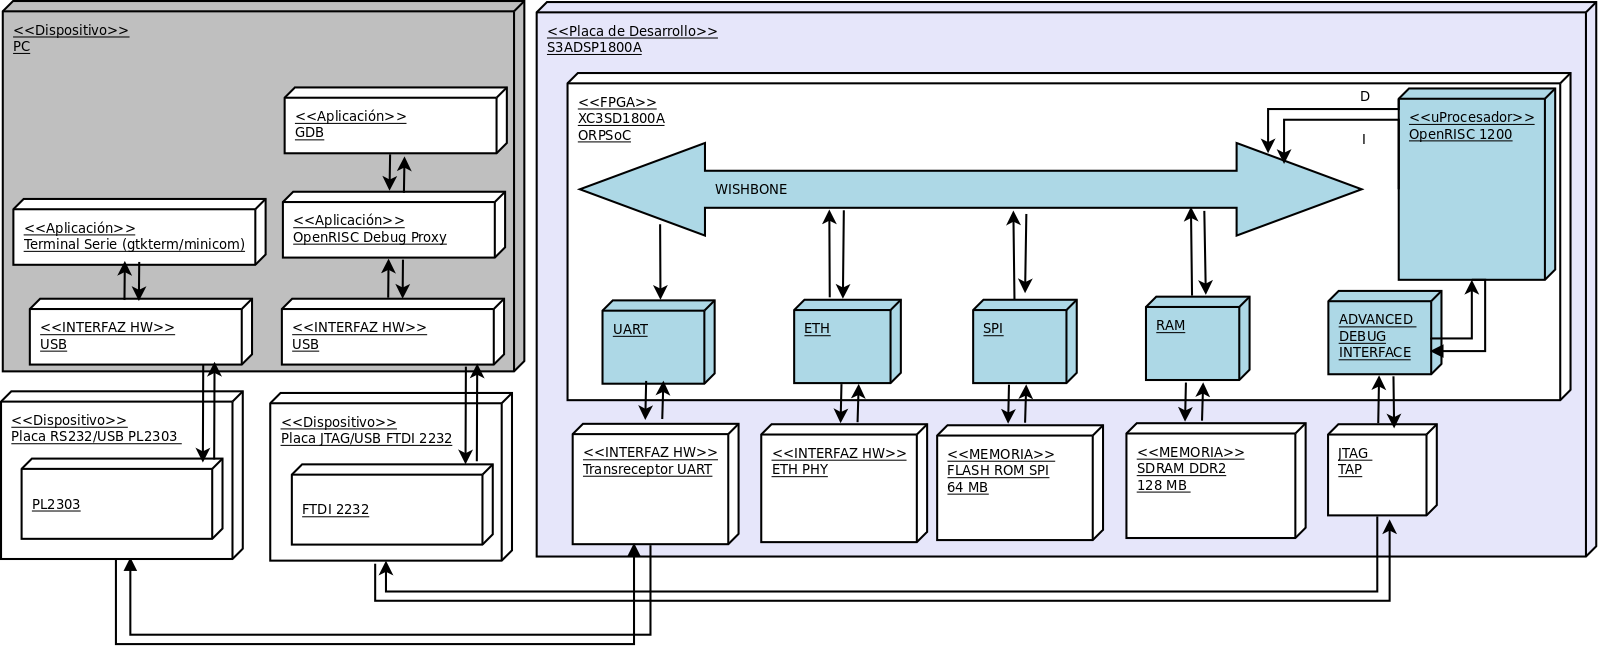
\includegraphics[width=1\textwidth,keepaspectratio=true]{./images/orpsoc}
  		\caption{Arquitectura Prototipo Dos}
  		\label{fig:orpsoc} 
 		\end{center}
		\end{figure}
	
		\section{Implementación}

		La implementación se realiza normalmente en cinco pasos básicos: 
		\begin {itemize}
		\item Descarga del script de instalación.
		\item Ejecución del script de instalación.
		\item Configuración de la placa especifica para la síntesis.
		\item Generación del flujo de bits.
		\item Programación de la FPGA Spartan 3a.
 		\end {itemize}
 
 Consulte la Guía de ORPSoC en el Anexo ~\ref{app:apendice2} para una comprensión más profunda de los pasos a seguir en la implementación sobre la
 placa de desarrollo S3ADSP1800A.

El módulo de Debug proporciona soporte para la depuración via JTAG. Se conectan al sistema mediante un Bus Wishbone: un modulo de RAM que provee acceso a las memorias SDRAM on board de la placa S3ADSP1800A, un módulo SPI que interactúa con la memoria flash on board de la placa antes mencionada, un módulo UART y un módulo ETHERNET. 
		


%%%%%%%%%%%%%%%%%%%%%%%%%%%%TESTING DOS
\newpage
		\section{Testing}

		\begin{table}[h!]
		\centering
		\begin{tabular}{ p{5cm} p{10cm}  }
		\hline 
		\rowcolor[gray]{0.8}  Caso de Prueba&  Interactuar correctamente con las interfaces hardware de Ethernet\\
		\hline 
		Código de Requerimiento & RQX-PB 2 , RQX-PB 3\\ 
		\hline 
		Requerimiento  &El prototipo debe garantizar el correcto funcionamiento de todos los periféricos conectados al SoC mediante el bus Wishbone\\ 
						&  El prototipo debe Interactuar correctamente con las interfaces hardware soportadas de la placa de desarrollo S3ADSP1800A\\
		\hline 
		Código de Testing & T008\\ 
		\hline
		Propósito &  El envío de paquetes echo del protocolo ICMP desde el SoC  \\
		\hline
		Realizado Por & Gomez, Pablo \\
		\hline	
		Entorno de Ejecución & Bare Metal \\
		\hline
		Precondiciones & \begin {itemize}
							\item Instanciación en la FPGA del SoC.
							\item Ejecución de una terminal serie en la PC
							\item Ejecución de una aplicación snifer en la PC
							\item Comunicación establecida entre la placa de desarrollo y la PC
							\item Herramientas de compilación cruzada funcionando correctamente
							\item Programas de prueba compilados correctamente
							\end {itemize} \\
		\hline
		Secuencia de Ejecución &  Ejecutación de la aplicación de prueba ethmac-ping.or32\\
		\hline
		Postcondiciones &  El programa de prueba ejecutándose sobre la RAM de la plataforma, lo que se manifiesta en la impresión de pantalla de la terminar serie en la PC y en los paquetes captados por la aplicación wireshark \\
		\hline
 		\multicolumn{2}{>{\columncolor[gray]{.8}}c}{Resultados}\\
		\hline
		Resultados Esperados & Poder observar por la terminal serial una cadena de string indicando el inicio del envío de paquetes ICMP y verificar la llegada de los mismos por medio de una aplicación ICMP \\
		\hline	
		Resultados Obtenidos & Al ejecutarse el programa de prueba pudo observarse la cadena mostrada en la Referencia ~\ref{lst:reseth}\\
		\hline
		\end{tabular}
		\end{table}


\begin{lstlisting}[frame=single,caption={Salida de la terminal serie durante la ejecución del programa ethmac-ping.or32},label={lst:reseth}]
eth ping program
board IP "192.168.1.2
\end{lstlisting}


\newpage


		\begin{table}[h!]
		\centering
		\begin{tabular}{ p{5cm} p{10cm}  }
		\hline 
	    \rowcolor[gray]{0.8}  Caso de Prueba&Interactuar correctamente con la memoria RAM. \\
		\hline 
		Código de Requerimiento & RQX-PB 4 \\ 
		\hline 
		Requerimiento  &  Se debe garantizar el acceso a las memorias RAM DDR2 de la plataforma S3ADSP1800A\\ 	

		\hline 
		Código de Testing & T007\\ 
		\hline
		Propósito & Comprobación del correcto funcionamiento del módulo de RAM implementado en el SoC\\
		\hline
		Realizado Por & Lovaisa Michelini, Valeria \\
		\hline	
		Entorno de Ejecución & Bare Metal \\
		\hline
		Precondiciones &  \begin {itemize}
							\item Instanciación del SoC en la FPGA.
							\item Ejecución de una terminal serie en la PC
							\item Comunicación establecida entre la placa de desarrollo y la PC
							\item Herramientas de compilación cruzada funcionando correctamente
							\item Programas de prueba compilados correctamente
							\end {itemize}\\
		\hline
		Secuencia de Ejecución & Ejecutación de la aplicación de prueba sdra-row.or32 \\
		\hline
		Postcondiciones & ORPSoC corriendo sobre FPGA, y la aplicación ejecutándose sobre la memoria RAM lo que se manifiesta en la impresión de pantalla de la terminar remota en la PC\\
		\hline
 		\multicolumn{2}{>{\columncolor[gray]{.8}}c}{Resultados}\\
		\hline
		Resultados Esperados & Poder observar por la terminal serial una cadena de string.\\
		\hline	
		Resultados Obtenidos & Al ejecutarse la aplicación de prueba de RAM sdra-row.o32 se pudo observar la cadena de string esperada "TEST OK!" \\
		\hline
		\end{tabular}
		\end{table}


\newpage
		\begin{table}[h!]
		\centering
		\begin{tabular}{ p{5cm} p{10cm}  }
		\hline 
		\rowcolor[gray]{0.8}  Caso de Prueba& Ejecución de la aplicación compilada en modo debug para números primos\\
		\hline 
		Código de Requerimiento & RQX-PA 5\\ 
		\hline 
		Requerimiento  & El prototipo debe ser capaz de ejecutar programas con capacidad de depuración generados mediante compilación cruzada en una arquitectura x86 y/o x86-64 para arquitectura la Open-RISC\\ 
		\hline 
		Código de Testing & T0011\\ 
		\hline
		Propósito &  Compilación en modo debug y Ejecución de un programa de calculo de números primos en c.
\\
		\hline
		Realizado Por & Gomez, Pablo \\
		\hline	
		Entorno de Ejecución & Bare Metal \\
		\hline
		Precondiciones &\begin {itemize}
							\item Instanciación en la FPGA del SoC.
							\item Ejecución de una terminal serie en la PC
							\item Descarga e instalación del complicador cruzado 
							\item Comunicación establecida entre la placa de desarrollo y la PC
							\item Herramientas de compilación cruzada funcionando correctamente
							\item Programas de prueba compilados correctamente
							\end {itemize}
 \\
		\hline
		Secuencia de Ejecución & Ejecución de la aplicación  numprim.or32\\
		\hline
		Postcondiciones & Aplicación corriendo sobre el ORPSoC instanciado en la FPGA, lo que se manifiesta en la impresión de pantalla de los números primos \\
		\hline
 		\multicolumn{2}{>{\columncolor[gray]{.8}}c}{Resultados}\\
		\hline
		Resultados Esperados & Poder observar por la terminal serial el resultado de la ejecución de la aplicación \\
		\hline	
		Resultados Obtenidos & Al ejecutarse el programa contador de nuemros primos pudo observarse la salida mostrada en la Referencia ~\ref{lst:rescom}\\
		\hline
		\end{tabular}
		\end{table}

\begin{lstlisting}[frame=single,caption={Salida de la terminal serie durante la ejecución del programanumprim.or32},label={lst:rescom}]
tiempo de ejecución:
cantidad de numeros primos entre 1 y 2000:
\end{lstlisting}


\newpage
		\begin{table}[h!]
		\centering
		\begin{tabular}{ p{5cm} p{10cm}  }
		\hline 
	    \rowcolor[gray]{0.8}  Caso de Prueba&  Ejecución del Benchmark CoreMark\\
		\hline 
		Código de Requerimiento & RQX-PB 7\\ 
		\hline 
		Requerimiento  &  El prototipo debe ser evaluado mediante el benchmark CoreMark para el posterior análisis de las capacidades del SoC\\ 
		\hline 
		Código de Testing & T009\\ 
		\hline
		Propósito & Medir el rendimiento de la unidad central de procesamiento embebida en el SoC\\ 
		\hline
		Realizado Por & Lovaisa Michelini, Valeria \\
		\hline	
		Entorno de Ejecución & Bare Metal \\
		\hline
		Precondiciones &  \begin {itemize}
							\item Instanciación del SoC en la FPGA.
							\item Ejecución de una terminal serie en la PC
							\item Comunicación establecida entre la placa de desarrollo y la PC
							\item Herramientas de compilación cruzada funcionando correctamente
							\item Programa coremark compilado correctamente
							\end {itemize}\\
		\hline
		Secuencia de Ejecución & Ejecución de la aplicación coremark.exe \\
		\hline
		Postcondiciones & ORPSoC corriendo sobre FPGA, lo que se manifiesta en la impresión de pantalla de la terminar serial en la PC de los resultados del programa de prueba \\
		\hline
 		\multicolumn{2}{>{\columncolor[gray]{.8}}c}{Resultados}\\
		\hline
		Resultados Esperados & Poder observar por la terminal serial los resultados de medición de performance.\\
		\hline	
		Resultados Obtenidos & Al ejecutarse la aplicación coremark.exe se pudo observar ~\ref{lst:rescrm} \\
		\hline
		\end{tabular}
		\end{table}


\begin{lstlisting}[frame=single,caption={Salida de la terminal serie de los resultados de la ejecución del benchmark},label={lst:rescrm}]
 ACA VA EL RESULTADO DE CORE MARK
\end{lstlisting}

		\section{Conclusión}

\chapter{Prototipo Tres : Implementación del SoC ORPSoC en FPGA con Sistema Operativo eCos}
		\section{Introducción}

		Para el tercer prototipo se añadió al prototipo dos la funcionalidad aportada por el Sistema Operativo de tiempo real eCos(embedded configurable operating system) que adiciona la capacidad de la ejecución de múltiples hilos. 


		\section{Requerimientos del prototipo}

		\begin{table}[h!]
		\centering		
		\begin{tabular}{ p{2.5cm} p{8cm} p{3cm} }
		\hline 
		\rowcolor[gray]{0.8} N\textordmasculine Req & Descripción\\
		\hline 
		RQX-PC 1 & El prototipo debe implementar un sistema operativos de tiempo real\\ 
		\hline 
		RQX-PC 2 & Se debe garantizar el correcto funcionamiento de todos los periféricos utilizando los driver y librerías provistas por el SO \\ 
		\hline 
		RQX-PC 3 & Se debe poder ejecutar programas que requiere la ejecución de múltiples hilos  \\ 
		\hline
		RQX-PC 4 & Se requiere la ejecución de programas de prueba para determinar las limitaciones en la ejecución de hilos \\ 
		\hline		
		\end{tabular}
		\end{table}
		

		\section{Matriz de Riesgo para el Prototipo Tres} 

		\begin{table}[h!]
		\centering
		\begin{tabular}{ p{2.5cm} p{9cm} p{2cm} p{2cm} }
		\hline 
		\rowcolor[gray]{0.8} N\textordmasculine Req Asociados& Riegos Asociados & Severidad  & Ocurrencia \\
		\hline
		RQX-PC 1& Fallas en la generación de la imagen del SO para ser montada en el SoC & Crítica       & Probable \\
		\hline				
				& Falta de documentación de apoyo para la implentación del SO bajo licencias de Software Libre & Crítico & Ocasional\\	
		\hline				
				 & Limitaciones para la ejecución de SO de tiempo real & Crítico & Ocasional\\	
 		
 		\hline	
		RQX-PC 2 	& Librerías necesarias inexistentes o con fallos& Crítico & Ocasional\\	
		
		\hline				
 					 & Drivers necesarios inexistentes o con fallos  & Severo  &  Ocasional\\ 
		\hline	
 		RQX-PC 3	&Problemas en la compilación e instalación de las herramientas de desarrollo de software& Severo  &  Ocasional\\ 
		\hline
		RQX-PB 4 & Problemas con el compilador para la generación del binario del programa de prueba  & Crítico&  Ocasional\\
		\hline
		\end{tabular}
		\caption{Tabla de Riegos vs. Requerimientos}
		%\label{tab:riegos}
		\end{table}

\newpage

 		\begin{table}[h!]
		\centering
		\begin{tabular}{ p{4cm} p{4cm} p{4cm} p{3cm} }
		\hline 
		\rowcolor[gray]{0.8} Riesgo & Consecuencia & Estrategia preventiva & Estrategia de contingencia\\
		\hline
		Fallas en la generación de la imagen del SO para ser montada en el SoC &Retraso en los tiempos de implementación.& Análisis previo de guías de resolución de problemas y preguntas frecuentes & Revisión de código y consulta a los desarrolladores\\		 
		\hline
		Falta de documentación de apoyo para la implentación del SO bajo licencias de Software Libre& Perdida de tiempo en realizar la implementación del SO & Revisión previa de la documentación existente para la elección del
SO & Dedicación de mayor tiempo para la implementación\\ 
		\hline
		 Limitaciones para la ejecución de SO de tiempo real & Inviabilidad para la ejecución
de aplicaciones en tiempo real & Análisis de los RTOS &Modificación del SO para el cumplimiento de las capacidades de ejecución en tiempo real\\
		\hline
		Librerías necesarias inexistentes o con fallos& Imposibilidad de desarrollo de aplicaciones para ejecutar sobre el SO de tiempo real& Análisis previo de las librerías disponibles y revisión de posibles bugs informados SO & Desarrollo de las librerías necesarias o corrección de errores\\			
		\hline
		Drivers necesarios inexistentes o con fallos & Imposibilidad de utilización
de los dispositivos necesarios&Análisis previo de los driver de los dispositivos a utilizar& Desarrollo de los drivers necesarios\\		
		\hline
		 Problemas en la compilación e instalación de las herramientas de desarrollo de software & Imposibilidad de desarrollo de aplicaciones que se ejecuten sobre el SO& Verificar la posibilidad de ejecución de las herramientas
en diferentes SO & Utilización de las herramientas en alguno de los SO compatibles\\
		\hline
		 Problemas con el compilador para la generación del binario del programa de prueba& Imposibilidad de medir las limitaciones en la ejecución de hilos & Consulta previa a la documentación del SO y guías de preguntas frecuentes & Depuración de código de prueba\\
		\hline
		\end{tabular}
		\caption{Planificación de riesgos}
		%\label{tab:planificación}
		\end{table}

\newpage
		
		\section{Descripción de la Estructura del Prototipo Tres}
		La Figura ~\ref{fig:ecos} muestra el diagrama de despliegue del prototipo tres. Este prototipo utiliza como base al prototipo dos pero se ejecutan 
		aplicaciones compiladas bajo ecOS.
		
		\begin{figure}[h!]
 		\begin{center}
  		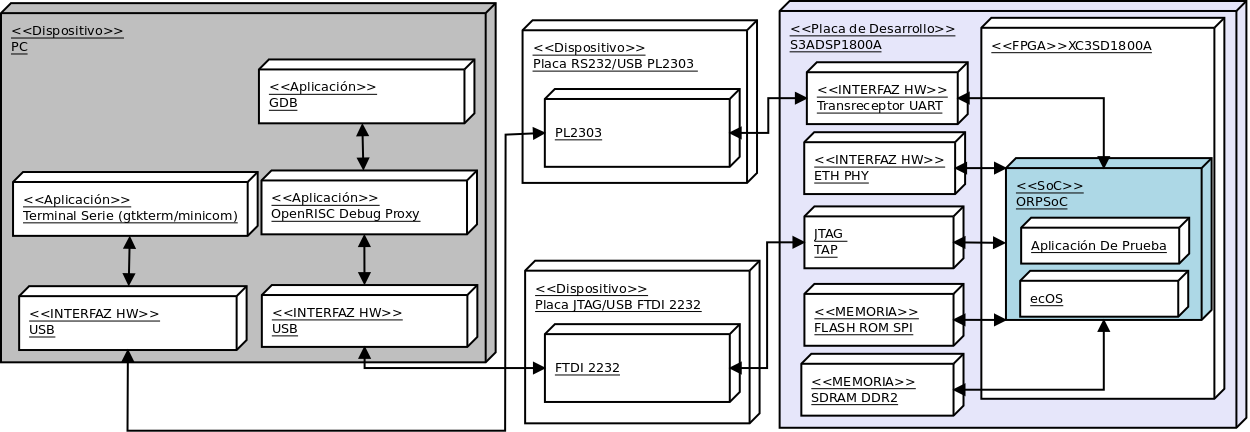
\includegraphics[width=1\textwidth,keepaspectratio=true]{./images/ecos}
  		\caption{Diagrama de Despliegue del Prototipo Tres}
  		\label{fig:ecos} 
 		\end{center}
		\end{figure}
	
		\section{Implementación}	
		
		\newpage
		
		\section{Testing}

		\begin{table}[h!]
		\centering
		\begin{tabular}{ p{5cm} p{10cm}  }
		\hline 
		\rowcolor[gray]{0.8}  Caso de Prueba &  Interactuar correctamente con la interfaz UART\\
		\hline 
		Código de Requerimiento & RQX-PC 2\\ 
		\hline 
		Requerimiento & Se debe garantizar el correcto funcionamiento de todos los periféricos utilizando los driver y librerías provistas por el SO \\ 
		\hline 
		Código de Testing & T012\\ 
		\hline
		Propósito &  Comprobación del correcto funcionamiento del componente UART\\
		\hline
		Realizado Por & Gomez, Pablo \\
		\hline	
		Entorno de Ejecución & SO - ecOS\\
		\hline
		Precondiciones & \begin {itemize}
							\item Instanciación en la FPGA del SoC
							\item Ejecución de una terminal serie en la PC 
 							\item Comunicación establecida entre la placa de desarrollo y la PC
							\item Herramientas de compilación cruzada funcionando correctamente
							\item Sistema operativo correctamenta instalado
							\item Programas de prueba compilados correctamente
							\end {itemize} \\
		\hline
		Secuencia de Ejecución &  Ejecutación de la aplicación de prueba hello.elf\\
		\hline
		Postcondiciones &  El programa de prueba ejecutándose sobre el sistema operativo ecOS, lo que se manifiesta en la impresión de pantalla en la
		terminal serie de la PC\\
		\hline
 		\multicolumn{2}{>{\columncolor[gray]{.8}}c}{Resultados}\\
		\hline
		Resultados Esperados & Poder observar por la terminal serial una cadena de string \\
		\hline	
		Resultados Obtenidos & Al ejecutarse el programa de prueba pudo observarse la cadena string esperada "Hello, ecOS World"\\
		\hline
		\end{tabular}
		\end{table}

	\newpage			


		\begin{table}[h!]
		\centering
		\begin{tabular}{ p{5cm} p{10cm}  }
		\hline 
		\rowcolor[gray]{0.8}  Caso de Prueba& Ejecución de hilos\\
		\hline 
		Código de Requerimiento & RQX-PC 3 , RQX-PC 4\\ 
		\hline 
		Requerimiento  	&  Se debe poder ejecutar programas que requiere la ejecución de múltiples hilos\\
		\hline 
						&  Problemas con el compilador para la generación del binario del programa de prueba\\
		\hline 
		Código de Testing & T014\\ 
		\hline
		Propósito &  Compilación y ejecución de un programa de prueba que ejecute hilos\\
		\hline
		Realizado Por & Lovaisa, Valeria \\
		\hline	
		Entorno de Ejecución & SO - ecOS \\
		\hline
		Precondiciones &    \begin {itemize}
							\item Instanciación en la FPGA del SoC.
							\item Ejecución de una terminal serie en la PC
							\item Comunicación establecida entre la placa de desarrollo y la PC
							\item Herramientas de compilación cruzada funcionando correctamente
							\item Sistema operativo correctamenta instalado
							\item Programas de prueba compilados correctamente
							\end {itemize}
		\\
		\hline
		Secuencia de Ejecución & Ejecución de la aplicación de prueba twothreads.elf \\
		\hline
		Postcondiciones & Aplicación ejecutándose sobre el sistema operativo \\
		\hline
 		\multicolumn{2}{>{\columncolor[gray]{.8}}c}{Resultados}\\
		\hline
		Resultados Esperados & Poder observar por la terminal serie el resultado de la ejecución de la aplicación\\
		\hline	
		Resultados Obtenidos & Al ejecutarse el programa de prueba de hilos pudo observarse la salida mostrada en la Referencia ~\ref{lst:salhilos} \\
		\hline
		\end{tabular}
		\end{table}

\begin{lstlisting}[frame=single,caption={Salida de la ejecución del programa de prueba twothreads},label={lst:salhilos}]
 ACA VA EL RESULTADO DE LA EJECUCIÓN DE HILOS
\end{lstlisting}

		\section{Conclusión}

\chapter{Prototipo Cuatro : Implementación del SoC ORPSoC en FPGA con Sistema Operativos Linux}
		\section{Introducción}
		El núcleo Linux, combinado con un conjunto utilidades de software libre, puede ajustarse al espacio limitado de hardware 
	    de los sistemas embedidos. Una instalación típica de un Linux embebido ocupa en promedio 2 MB. En el prototipo cuatro se utilizó una versión
	    reducida del núcleo de Linux y herramientas provistas por el paquete BusyBox. 
		
		\section{Requerimientos del prototipo}
		
		\begin{table}[h!]
		\centering	
		\begin{tabular}{ p{2.5cm} p{8cm} p{3cm} }
		\hline 
		\rowcolor[gray]{0.8} N\textordmasculine Req  & Descripción\\
		\hline                             	RQX-PD 1 & El prototipo debe implementar el sistema operativos Linux\\ 
		\hline  							RQX-PD 2 & Se requiere la instalación de un gestor de arraque que posibilite el inicio del sistema operativo\\ 
		\hline 								RQX-PD 3 & Se debe poder grabar como aplicación firmware el gestor de arranque en la memoria flash SPI de la placa de desarrollo\\
		\hline 								RQX-PD 4 & El prototipo debe tener capacidad de ejecución de aplicaciones sobre el sistema operativo Linux\\
		\hline 
		\end{tabular}
		\end{table}
		
		
		\section{Matriz de Riesgo para el Prototipo Cuatro} 

		\begin{table}[h!]
		\centering
		\begin{tabular}{ p{2.5cm} p{9cm} p{2cm} p{2cm} }
		\hline 
		\rowcolor[gray]{0.8} N\textordmasculine Req Asociados  & Riegos Asociados & Severidad  & Ocurrencia \\
		\hline RQX-PC 1 & Fallas en la generación de la imagen del SO para ser montada en el SoC & Crítica       & Probable \\
		\hline			& Falta de documentación de apoyo para la implentación del SO bajo licencias de Software Libre & Crítico & Ocasional\\	
		\hline			& Limitaciones para la ejecución de SO de tiempo real & Crítico & Ocasional\\	
 		\hline RQX-PC 2 & Librerías necesarias inexistentes o con fallos& Crítico & Ocasional\\	
		\hline			& Drivers necesarios inexistentes o con fallos  & Severo  &  Ocasional\\ 
		\hline RQX-PC 3	& Problemas en la compilación e instalación de las herramientas de desarrollo de software& Severo  &  Ocasional\\ 
		\hline RQX-PB 4 & Problemas con el compilador para la generación del binario del programa de prueba  & Crítico&  Ocasional\\
		\hline
		\end{tabular}
		\caption{Tabla de Riegos vs. Requerimientos}
		%\label{tab:riegos}
		\end{table}

		\newpage

 		\begin{table}[h!]
		\centering
		\begin{tabular}{ p{4cm} p{4cm} p{4cm} p{3cm} }
		\hline 
		\rowcolor[gray]{0.8} Riesgo & Consecuencia & Estrategia preventiva & Estrategia de contingencia\\
		\hline Errores en la configuración de compilación del kernel para el SoC utilizado & 
		       Retraso en los tiempos de implementación & 
		       Análisis previo de archivos de configuración del SoC seleccionado o similares & 
		       Revisión y correción de archivos de configuración\\
		\hline Fallas en la generación de la imagen del SO y/o el gestor arranque para ser montada en el SoC & 
		       Retraso en los tiempos de implementación & 
		       Análisis previo de guías de resolución de problemas y preguntas frecuentes & 
		       Revisión de código y consulta a los desarrolladores\\
		\hline Falta de documentación de apoyo para la implentación del SO y/o gestor de arranque para la arquitectura OpenRISC & 
		       Demoras en la implementación del SO & 
		       Revisión previa de la documentación existente y guías de resolución de problemas & 
		       Mayor inversión de tiempo para la implementación\\
		\hline Falta de soporte del SO Linux y/o el gestor de arranque para su implementación en el hardware disponible & 
			   Fallos en la ejecución del sistema operativo & 
		       Análisis previo de limitaciones en la documentación de los desarrolladores y guías de resolución de problemas & 
		       Revisión y desarrollo de código del SO necesario para proveer soporte al hardware\\
		\hline Librerías necesarias inexistentes o con fallos & 
			   Imposibilidad de desarrollo de aplicaciones para ejecutar sobre el SO &
			   Análisis previo de las librerías disponibles y revisión de posibles bugs informados SO & 
			   Desarrollo de las librerías necesarias o corrección de errores\\
		\hline Drivers necesarios inexistentes o con fallos & 
			   Imposibilidad de utilización de los dispositivos necesarios & 
			   Análisis previo de los driver de los dispositivos a utilizar & 
			   Desarrollo de los drivers necesarios\\		
		\hline Problemas en la compilación e instalación de las herramientas de desarrollo de software & 
			   Imposibilidad de desarrollo de aplicaciones que se ejecuten sobre Linux Embebido & 
			   Verificación previa de la documentación de los desarrolladores y guías de resolución de problemas & 
			   Revisión de codigo y corrección de errores\\
		\hline
		\end{tabular}
		\caption{Planificación de riesgos}
		%\label{tab:planificación}
		\end{table}

		\newpage
		
		\section{Descripción de la Estructura del Prototipo Cuatro}
		Se muestra a continuación (Figura ~\ref{fig:proto4}) el diagrama de despliegue del prototipo cuatro. Se utiliza como base nuevamente el prototipo
		dos con un sistema operativo linux ejecutándose en él.

		\begin{figure}[h!]
 		\begin{center}
  		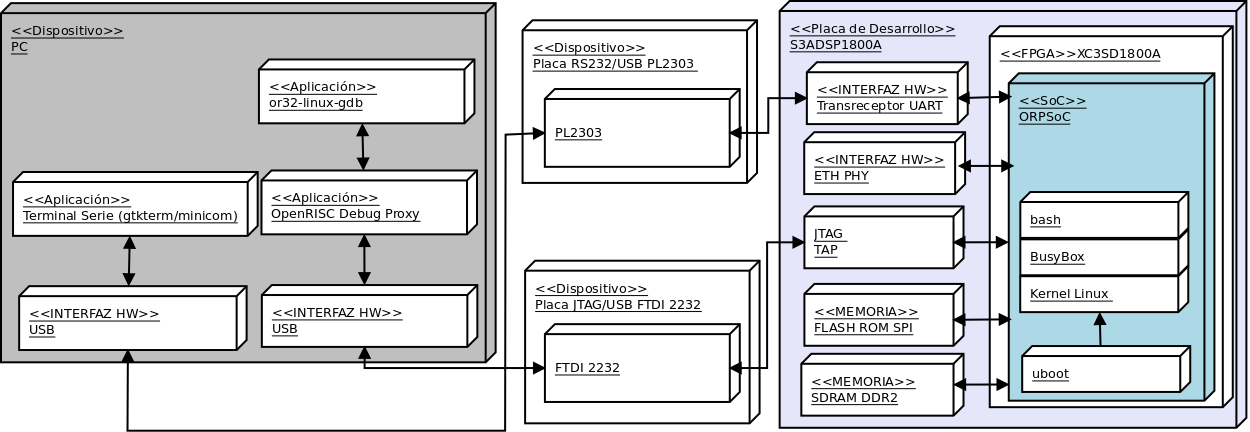
\includegraphics[width=1\textwidth,keepaspectratio=true]{./images/proto4}
  		\caption{Diagrama de Despliegue del Prototipo Cuatro}
  		\label{fig:proto4} 
 		\end{center}
		\end{figure}
	
		\newpage

		\section{Implementación}	
		
		\section{Testing}
		
		\begin{table}[h!]
		\centering
		\begin{tabular}{ p{5cm} p{10cm}  }
		\hline 
		\rowcolor[gray]{0.8} 	 Caso de Prueba & Carga de programa mediante el gestor de arranque UBoot\\
		\hline  		Código de Requerimiento & RQX-PD 2\\ 
		\hline  				  Requerimiento & Se requiere la instalación de un gestor de arraque que posibilite el inicio del sistema operativo\\
		\hline 				  Código de Testing & T015\\ 
		\hline 						  Propósito & Comprobación del correcto funcionamiento del gestor de arranque\\
		\hline					  Realizado Por & Lovaisa, Valeria \\
		\hline	 		   Entorno de Ejecución & Bare Metal\\
		\hline		   		   	 Precondiciones & \begin {itemize}
												  \item Instanciación en la FPGA del SoC ORPSoC
												  \item Ejecución de una terminal serie en la PC 
 												  \item Comunicación establecida entre la placa de desarrollo y la PC mediante Serial y eth
 												  \item Servidor TFTP funcionando correctamente sobre el SO host
												  \item Herramientas de compilación cruzada funcionando correctamente
												  \item Gestor de arranque y aplicación de prueba compilados correctamente
												  \item Imagen de arranque sin errores
												  \end {itemize} \\
		\hline			 Secuencia de Ejecución &  Ejecutación de la aplicación de prueba numprim.or32 a través de Uboot\\
		\hline					Postcondiciones &  El gestor de arranque inicia correctamente el programa de prueba, lo que se manifiesta en la impresión de la salida
		del gestor de arranque y el programa prueba en la terminal serie de la PC\\
		\hline	\multicolumn{2}{>{\columncolor[gray]{.8}}c}{Resultados}\\
		\hline			   Resultados Esperados & Poder observar por la terminal serial las salida de los programas \\
		\hline	 		   Resultados Obtenidos & Al ejecutarse el programa de prueba pudo observarse la salida mostrada en la Referencia ~\ref{lst:salidauboot}\\
		\hline	
		\end{tabular}
		\end{table}
		
\begin{lstlisting}[frame=single,caption={Salida de la ejecución del programa de prueba cargado por uboot},label={lst:salidauboot}]
 ACA VA EL RESULTADO DE CORRER UN PROGRAMA MEDIANTE UBOOT
\end{lstlisting}
		
		\begin{table}[h!]
		\centering
		\begin{tabular}{ p{5cm} p{10cm}  }
		\hline 
		\rowcolor[gray]{0.8} 	 Caso de Prueba & Inicio del gestor de arranque desde la memoria Flash SPI\\
		\hline  		Código de Requerimiento & RQX-PD 3\\ 
		\hline  				  Requerimiento & Se debe poder grabar como aplicación firmware el gestor de arranque en la memoria flash SPI de la placa de desarrollo\\
		\hline 				  Código de Testing & T016\\ 
		\hline 						  Propósito & Verificación del inicio del gestor de arranque almacenado en la Flash SPI \\
		\hline					  Realizado Por & Lovaisa, Valeria \\
		\hline	 		   Entorno de Ejecución & Bare Metal\\
		\hline		   		   	 Precondiciones & \begin {itemize}
												  \item Instanciación en la FPGA del SoC ORPSoC
												  \item Ejecución de una terminal serie en la PC 
 												  \item Comunicación establecida entre la placa de desarrollo y la PC mediante Serial
 												  \item Herramientas de compilación cruzada funcionando correctamente
												  \item Gestor de arranque compilado correctamente
												  \item Imagen del gestor de arranque almacenada en la memoria Flash SPI de la placa de desarrollo
												  \end {itemize} \\
		\hline			 Secuencia de Ejecución &  Arranque inicial o reset del hardware\\
		\hline					Postcondiciones &  El gestor de arranque inicia correctamente , lo que se manifiesta en la impresión de la salida
		del gestor de arranque en la terminal serie de la PC\\
		\hline	\multicolumn{2}{>{\columncolor[gray]{.8}}c}{Resultados}\\
		\hline			   Resultados Esperados & Poder observar por la terminal serial las salida del Uboot \\
		\hline	 		   Resultados Obtenidos & Al ejecutarse el programa de prueba pudo observarse la salida mostrada en la Referencia ~\ref{lst:salidaspi}\\
		\hline	
		\end{tabular}
		\end{table}
		
\begin{lstlisting}[frame=single,caption={Salida de la ejecución del programa de prueba cargado por uboot},label={lst:salidauboot}]
 ACA VA EL RESULTADO DE CORRER UBOOT DESDE LA SPI
\end{lstlisting}		
		
		\begin{table}[h!]
		\centering
		\begin{tabular}{ p{5cm} p{10cm}  }
		\hline 
		\rowcolor[gray]{0.8} 	 Caso de Prueba & Implementación del SO Linux Embebido\\
		\hline  		Código de Requerimiento & RQX-PD 1\\ 
		\hline  				  Requerimiento & El prototipo debe implementar el sistema operativos Linux\\
		\hline 				  Código de Testing & T017\\ 
		\hline 						  Propósito & Implementar correctamente un Sistema Operativo Linux Embebido sobre un SoC ORPSoC\\
		\hline					  Realizado Por & Lovaisa, Valeria \\
		\hline	 		   Entorno de Ejecución & Bare Metal\\
		\hline		   		   	 Precondiciones & \begin {itemize}
												  \item Instanciación en la FPGA del SoC ORPSoC
												  \item Ejecución de una terminal serie en la PC 
 												  \item Comunicación establecida entre la placa de desarrollo y la PC
 												  \item Herramientas de compilación cruzada funcionando correctamente
 												  \item Configuración del kernel adaptada al SoC
												  \item Imágen del Sistema Operativo Linux compilada correctamente 
												  \end {itemize}\\
		\hline			 Secuencia de Ejecución & Inicio del Sistema Operativo \\
		\hline					Postcondiciones & Se inicia correctamente el Sistema Operativo, lo que se manifiesta en la impresión de la salida
		de la secuencia de arranque de linux en la terminal serie de la PC\\
		\hline	\multicolumn{2}{>{\columncolor[gray]{.8}}c}{Resultados}\\
		\hline			   Resultados Esperados & Lograr observar por la terminal serial la secuencia de arranque del Sistema Operativo\\
		\hline	 		   Resultados Obtenidos & Al ejecutarse el programa de prueba pudo observarse la salida mostrada en la Referencia ~\ref{lst:sallinux}\\
		\hline	
		\end{tabular}
		\end{table}
		
\begin{lstlisting}[frame=single,caption={Salida de la secuencia de incio de Linux Embebido},label={lst:sallinux}]
 ACA VA EL RESULTADO DE CORRER UBOOT DESDE LA SPI
\end{lstlisting}		
		
		\begin{table}[h!]
		\centering
		\begin{tabular}{ p{5cm} p{10cm}  }
		\hline 
		\rowcolor[gray]{0.8} 	 Caso de Prueba & Ejecución de aplicaciones de prueba sobre Linux\\
		\hline  		Código de Requerimiento & RQX-PD 4\\ 
		\hline  				  Requerimiento & El prototipo debe tener capacidad de ejecución y depuración de aplicaciones sobre el sistema operativo Linux\\
		\hline 				  Código de Testing & T018\\ 
		\hline 						  Propósito & Ejecución de aplicaciones de prueba sobre entorno Linux\\
		\hline					  Realizado Por & Lovaisa, Valeria \\
		\hline	 		   Entorno de Ejecución & Linux\\
		\hline		   		   	 Precondiciones & \begin {itemize}
												  \item Instanciación en la FPGA del SoC ORPSoC
												  \item Ejecución de una terminal serie en la PC 
 												  \item Comunicación establecida entre la placa de desarrollo y la PC
 												  \item Herramientas de compilación cruzada para su ejecución sobre Linux funcionando correctamente
												  \item SO Linux ejecutándose correctamente sobre el SoC ORPSoC 
												  \end {itemize} \\
		\hline			 Secuencia de Ejecución & \begin {itemize}
						 					 	  \item Inicio del gestor de arranque
												  \item Inicio del Sistema Operativo
												  \item Ejecución de la aplicación de prueba
						 						  \end {itemize} \\
		\hline					Postcondiciones &  Se ejecuta correctamente el programa de prueba, lo que se manifiesta en la impresión de la salida
		del bash de linux en la terminal serie de la PC\\
		\hline	\multicolumn{2}{>{\columncolor[gray]{.8}}c}{Resultados}\\
		\hline			   Resultados Esperados & Poder observar por la terminal serial las salida de ejecución del programa de prueba \\
		\hline	 		   Resultados Obtenidos & Al ejecutarse el programa de prueba pudo observarse la salida mostrada en la Referencia ~\ref{lst:salidalinux}\\
		\hline	
		\end{tabular}
		\end{table}

\begin{lstlisting}[frame=single,caption={Salida de la ejecución del programa de prueba ejecutado en Linux Embebido},label={lst:salidalinux}]
 ACA VA EL RESULTADO DE CORRER UBOOT DESDE LA SPI
\end{lstlisting}		
		
		\section{Conclusión}
